\documentclass[a4paper, 12pt]{article}
\usepackage[utf8]{inputenc}
\usepackage[brazilian]{babel}
\usepackage{indentfirst}
\usepackage{graphicx}
\usepackage{float}
\usepackage{titlesec}
\usepackage{amsmath}
\usepackage{caption}
\usepackage{subfigure}
\usepackage{hyperref}
\usepackage{fixltx2e} %Para subscripts
\usepackage{pgfplots}
\usepackage{textcomp}
\usepackage{enumitem}

\titlelabel{\thetitle. \quad}
\newcommand{\tab}{\hspace{2cm}}


\title{}
\author{}

\begin{document}
    \begin{center}
	   \begin{figure}
		   \centering
		   
\includegraphics[scale=1.0]{ufrn.jpg}
	   \end{figure}
		UNIVERSIDADE FEDERAL DO RIO GRANDE DO NORTE\\
		CENTRO DE TECNOLOGIA\\
		DEPARTAMENTO DE COMPUTAÇÃO E AUTOMAÇÃO\\
		DISCIPLINA DE INTELIGÊNCIA ARTIFICIAL APLICADA
	\end{center}
	\vspace{1cm}
	\begin{center}
		\Large \textbf{Prova 3}\\
		\small \textit{Eric Calasans de Barros - 20170155390\\José Genilson da Silva Filho - 20170155603}
	\end{center}
	
	\section{Questão 1}
	Para a função em questão, a saber $f(x) = x^{3} + x^{2} + 1$, segundo o gráfico abaixo, observa-se que o mínimo global encontra-se em $-\infty$.  Plotando o gráfico no intervalo [-2:2]:
		\begin{center}
			\begin{tikzpicture}% function
			\begin{axis}
				[xlabel=x,
				domain=-2:2,
				ylabel=f(x),
				ymin=-10,
				ymax=10,
				axis x line=center,
				axis y line=center]
				\addplot [smooth, mark=none, color=red] {x^3+x^2+1};
			\end{axis}
			\end{tikzpicture}
		\end{center}
	Para encontrar o mínimo local, podemos utilizar uma estratégia de \textbf{BUSCA EM PROFUNDIDADE}, com a seguinte estratégia:  utilizando uma estrutura de árvore, começaríamos a busca pela raiz e, partindo da extremidade direita do espaço de busca(limite superior), percorreríamos este espaço escolhendo aleatoriamente outros pontos, os quais se configurariam em novos nós da árvore.  A cada novo nó seria verificado se este é maior ou menor que o anterior:  em sendo maior ele ficaria à direita do nó raiz;  sendo menor, à esquerda.  O processo seria repetido até que se chegasse ao último nó à esquerda, o qual seria o mínimo local.
	
	\section{Questão 2}
	No algoritmo \textbf{A* (A-estrela)}, temos uma matriz que deve ser considerada como um grafo, onde os elementos da matriz são os nós do grafo e cada nó são ligados com seus vizinhos (laterais e diagonais). Os elementos vizinhos tem um custo associado.
	Existem dois tipos de peso: o peso G é referente ao custo em relação do elemento anterior até o elemento seguinte e o peso H é em relação ao elemento que se pretende chegar, e por último temos o custo \textbf{F} que é dado por $F = G + H$. Os custos considerados na questões foram de 10 para movimentos na horizontal e na vertical e foi considerado 15.\\
	
	Iremos utilizar a técnica de Manhattan para o cálculo de H, que é calculado contando apenas o pesos para chegar no destino só movimentando horizontalmente e verticalmente e ignorando as paredes. No nosso exemplo temos um H com peso 90 do elemento inicial da matriz até o elemento marcado como o final. Abaixo tem um modelo de como os pesos e o pai do nó seguinte serão mostrados na tabela:
		\begin{figure}[H]
			\centering
			
\includegraphics[width=0.4\linewidth]{1}
		\end{figure}
	A seta vermelha indica de onde o caminho está vindo para chegar no elemento atual.
		\begin{figure}[H]
			\centering
			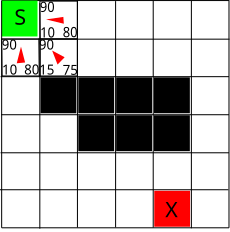
\includegraphics[width=0.4\linewidth]{2}
		\end{figure}
	Cada elemento vizinho terá os seus pesos, e uma seta que aponta para o elemento anterior que descobriu os adjacentes. Esse ponteiro é importante para no fim da execução das iterações, a gente ter o caminho completo.
		\begin{figure}[H]
			\centering
			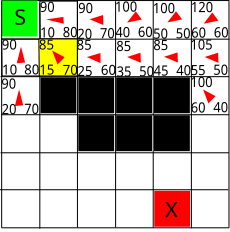
\includegraphics[width=0.4\linewidth]{3}
		\end{figure}
	Como vemos na imagem acima, o ponto que chegamos seguindo por esse caminho já não é o que possui o menor peso associado, logo podemos buscar um outro caminho com um peso menor que o atual, vamos então escolher o possível caminho atingido pelo quadrado vizinho logo a abaixo de S para continuar a busca no algoritmo.
		\begin{figure}[H]
			\centering
			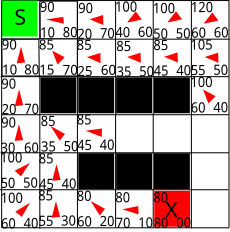
\includegraphics[width=0.4\linewidth]{4}
		\end{figure}
	Finalmente encontramos o ponto final, pelo algoritmo, vemos que o peso F encontrado é de 80, no próximo passo é feito um backtracking para marcar o caminho até o início, é aí que o ponteiro entra em cena, ele é utilizado para recuperar a informação do pai e assim de quadrado em quadrado montamos o caminho de retorno, para exemplificar marcamos o caminho com círculos azuis:
		\begin{figure}[H]
			\centering
			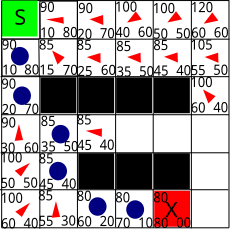
\includegraphics[width=0.4\linewidth]{5}
		\end{figure}
	Realmente o algoritmo retornou uma ótima solução para o problema, apesar de demorar um pouco para executar todas as etapas do algoritmo, mas encontrou uma solução satisfatória.
	
	\section{Questão 3}
	Dada a função $y = x_{1}^{2} - 2x_{1}x_{2} + 6x_{1} + x_{2}^2 - 6x_{2}$, deseja-se otimizá-la, ou seja, encontrar seu máximo ou mínimo, conforme seja o caso, utilizando-se de algoritmos genéticos como recurso para tal, dada a não linearidade do problema em questão(algoritmos genéticos se configuram em uma boa ferramenta para situações como essa).  Em consulta através de \url{http://www.wolframalpha.com}, observamos que a função tem um mínimo global em \textbf{-9}, sendo este o alvo(\textit{target}) para ser obtido com o algoritmo genético.\\ 
	
	Utilizando o MATLAB\textregistered, através da \textbf{Optimization Tool Toolbox}, realizamos 12 experimentos variando os parâmetros exigidos na questão de forma que, a cada 2 experimentos nós variamos um parâmetro e mantivemos os outros nas configurações padrão da toolbox, a saber:
		\begin{itemize}
			\item Tamanho da população = 50;
			\item Taxa de cruzamento = 0.8;
			\item Elitismo = 0.05 ou 5\% da nova população é composta pelos melhores da anterior;
			\item Taxa de mutação = função \textbf{probabilidade gaussiana};
			\item Função de cruzamento = Máscara;
			\item Função de seleção = Amostragem Universal Estocástica
			\item Critério de parada = $100\times\text{número de variávies independentes(2)}$.  Pela função em questão, o algoritmo para na 200ª geração.
		\end{itemize}
	  Seguem os resultados e discussões:
		\begin{enumerate}[label=\alph*)]
			\item \textbf{Tamanho da população}\\
			Os experimentos foram realizados com 100 e 10 indivíduos respectivamente.  Com 50 indivíduos o algoritmo convergiu na 51ª geração;  com 10 indivíduos, convergiu na 83ª geração.  \textbf{Por este experimento podemos inferir que um maior número de indivíduos na população acelera a convergência.}
			\item \textbf{Taxa de cruzamento}\\
			Neste experimento alteramos a taxa de cruzamento, utilizando 0.2 e 0.9.  No primeiro caso o algoritmo achou o mínimo na 53ª geração enquanto que no segundo caso convergiu na 125ª geração.  Constatamos que uma taxa de cruzamento menor preserva as características da população mas isso por si só pode propiciar o surgimento de soluções em mínimos locais.  De alguma forma isso não aconteceu e o algoritmo achou o mínimo local em uma taxa de cruzamento menor.
			\item \textbf{Elitismo}\\
			Neste experimento resolvemos comparar uma taxa maior de elitismo(preservação dos melhores indivíduos para a próxima geração) em relação ao padrão da toolbox.  Com o padrão o algoritmo convergiu na 53ª geração;  com 30\% de elitismo o algoritmo convergiu na 164ª geração.  Preservando mais indivíduos da população original observamos que uma população "viciada" foi formada, dificultando a busca por novas soluções.
			\item \textbf{Taxa de mutação}\\
			Alteramos a função de mutação para uma \textbf{probabilidade uniforme} e setamos os valores de 0.01 e 0.1 como taxa de mutação.  Esse parâmetro é responsável diretamente por uma maior probabilidade de descaracterização do indivíduo, propiciando surgimento de "mutantes" e prejudicando a convergência.  Resolvemos mostrar esses resultados sob a forma de gráfico para visualizar melhor o efeito de descaracterização dos indivíduos, embora a convergência tenha sido a mesma.
				\begin{figure}[H]
					\centering
						\subfigure[Taxa de mutação de 0.01]{
							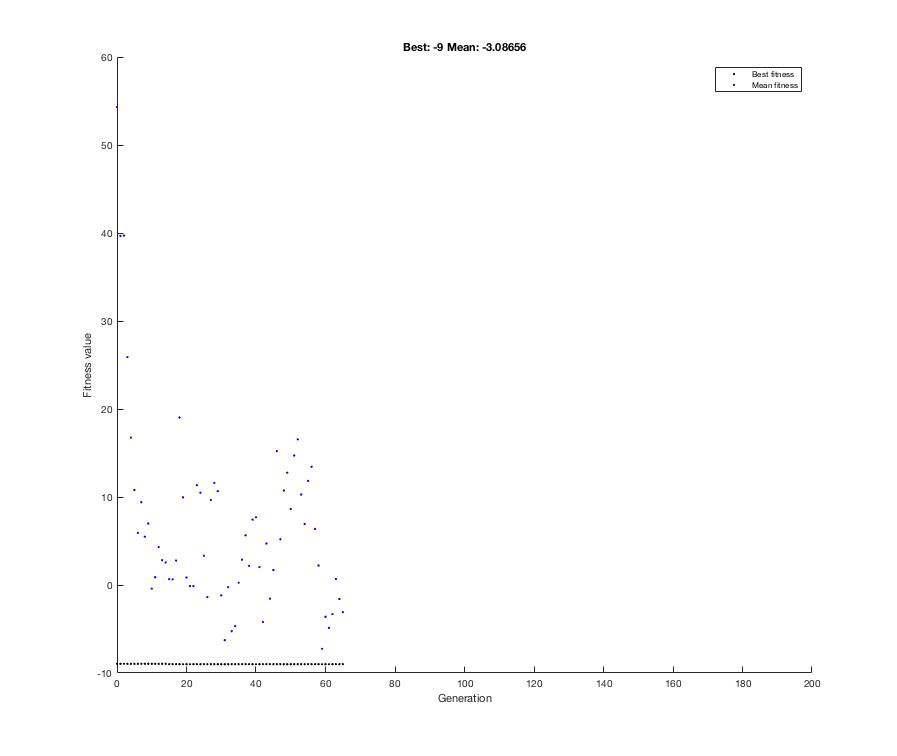
\includegraphics[width=60mm]{mut001}
						}
						~
						\subfigure[Taxa de mutação de 0.5]{
							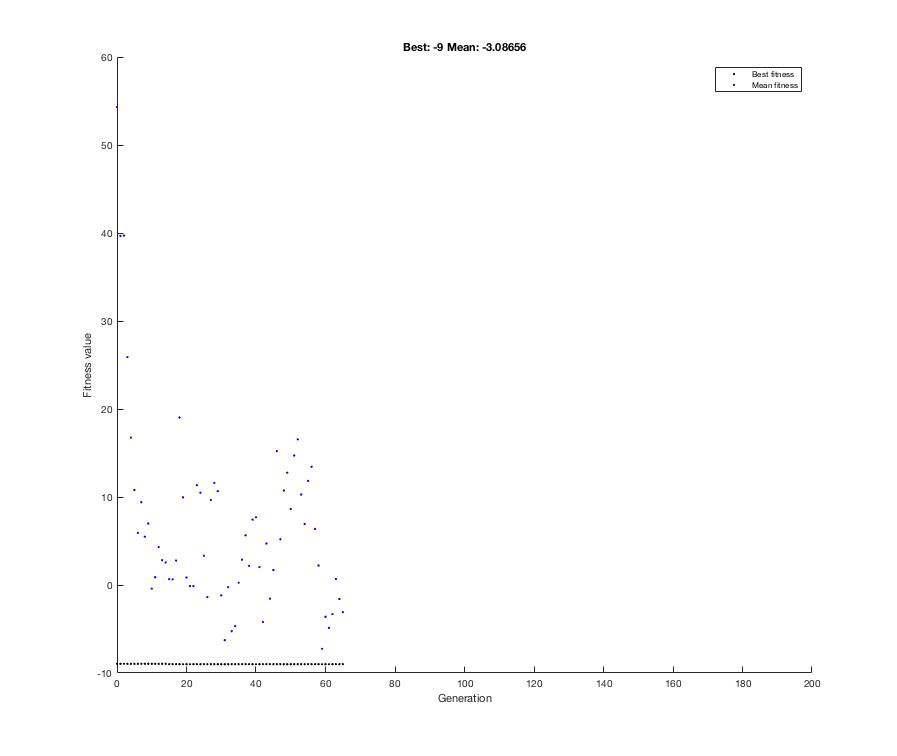
\includegraphics[width=60mm]{mut05}
						}
					\caption{Efeito de Descaracterização da População pela Taxa de Mutação}
				\end{figure}
			\item \textbf{Função de cruzamento}\\
			Mudando a função de cruzamento de Máscara para \textbf{Single Point} não constatamos mudanças na convergências: todas convergiram para praticamente o mesmo valor de mínimo:-8.99883978505099 para Máscara e -8.999982571355233 para Single Point.
			\item \textbf{Função de seleção}\\
			Testamos as funções \textbf{Roleta} e \textbf{Torneio} e não constatamos diferenças entre os dois modos de seleção.
		\end{enumerate}
	 
	\section{Questão 4}
		\begin{enumerate}[label=\alph*)]
			\item A \textbf{busca local} procura soluções na sua vizinhança, fazendo com que o processo de otimização ocorra mais rápido.  No entanto, esta estratégia de busca pode levar ao achado de mínimos locais, o que pode ser prejudicial caso este não seja o objetivo.  As \textbf{buscas heurísticas} obtém também um valor de mínimo baseado num espaço de busca definido ou não.  Também não há garantias de que o mínimo encontrado seja global ou local e a convergência pode demorar a ocorrer.
			\item Fácil implementação, convergência acelerada quando em conjunto com outros tipos de algoritmos de busca, heurísticos ou determinísticos.  A principal desvantagem é a possibilidade de convergência para pontos de mínimo locais, o que pode ser algo não desejável.
		\end{enumerate}
	
\end{document}